\section{Cenário}
\label{sec:cenario}
O cenário ``Levar compras'', que será explanado logo a seguir é idealizado no HNS da Figura \ref{fig:hnsworkmodel}. Neste, cada dispositivo da casa (veículo terrestre, elevador, garra mecânica) é disponibilizado como um serviço Web RESTFul. O HS deste cenário é um servidor Web RESTFul com um FIM (seção\ref{sec:featureinteraction}) integrado. A discussão do motivo de se utilizar dispositivos como serviços Web e, RESTFul em vez de SOAP foi realizada na seção \ref{subsec:dispositivosWeb}.

\begin{figure}[!htb] \centering 
  \centering
  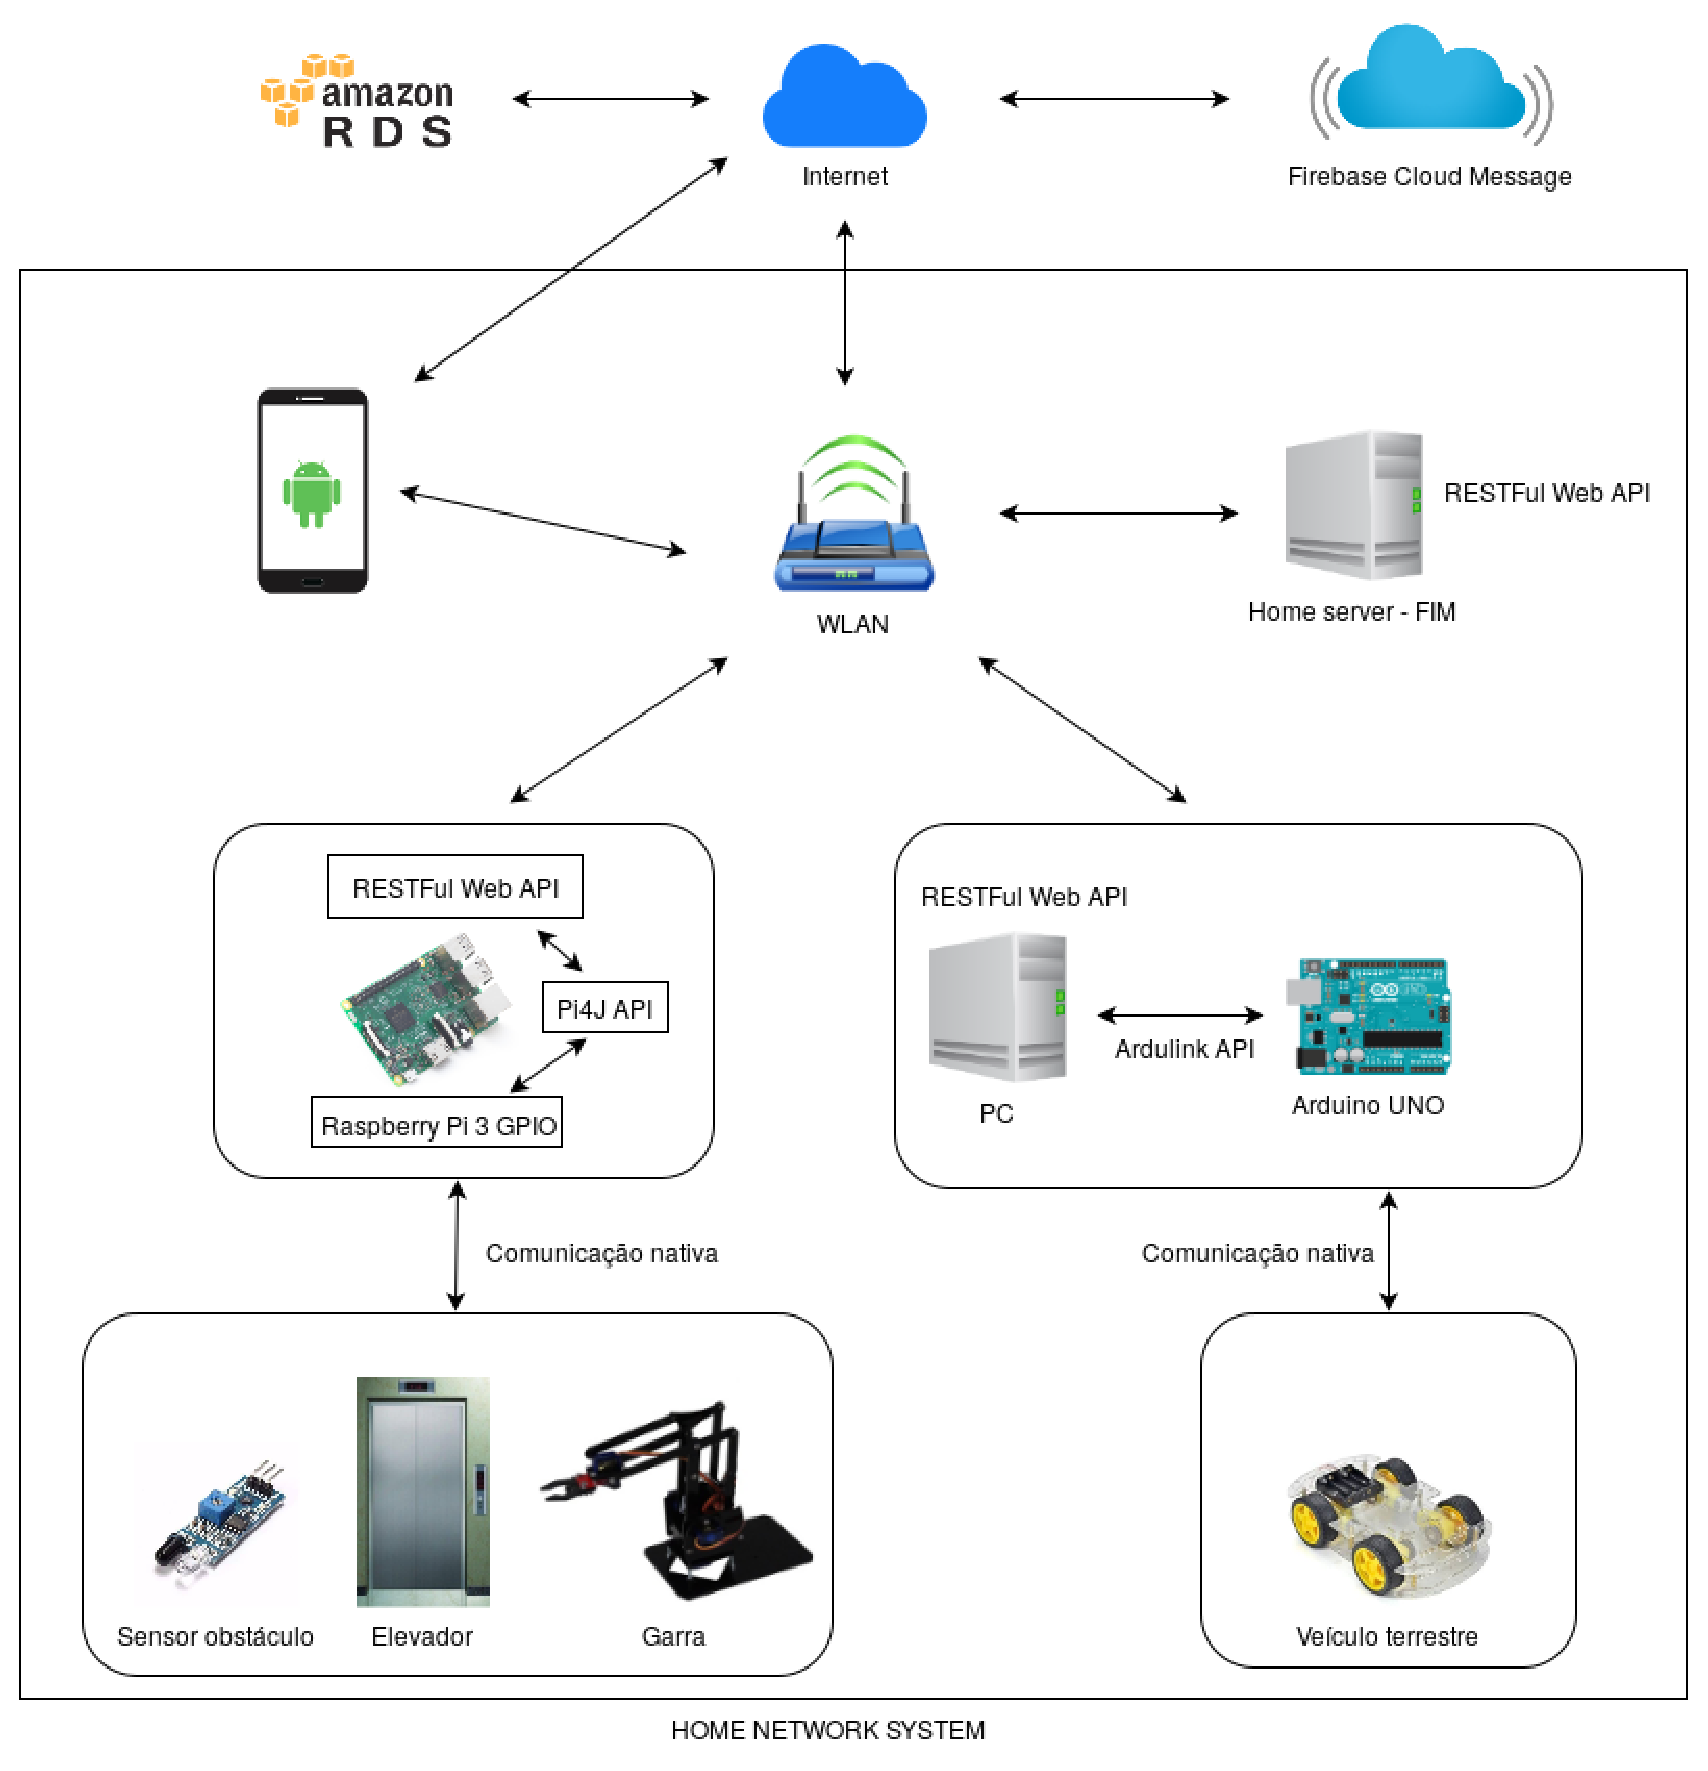
\includegraphics[width=1.0\columnwidth]{cenario} 
  \caption{Modelo do HNS utilizado neste trabalho.} 
  \label{fig:hnsworkmodel}
\end{figure}

O cenário ``Levar compras'' refere-se a funcionalidade (\textit{feature} ou característica)  oferecida pelo HS. Esta característica é provida através da composição dos serviços do elevador, veículo e garra. O cenário em questão pode ser visualizado na Figura \ref{fig:cenario} e é descrito a seguir.

\begin{enumerate}
\item Um usuário da casa (morador ou visitante), organiza as compras numa cesta (que tem formato expansível) e a coloca sobre o veículo terrestre.
\item O usuário então aciona o serviço ``Levar compras'' (disponibilizado pelo HS) através do seu \textit{smartphone}. O serviço então começa sua execução.
\item O FIM solicita informações de restrições do elevador e veículo terrestre, assim como quais objetos compõem a cesta. Este então verifica se a cesta colocada sobre o carro quebrou alguma restrição do mesmo e se a massa total dos objetos excedem a carga máxima do elevador.
\item Se nenhuma destas restrições foram quebradas o FIM solicita ao veículo terrestre que leve a as compras até as proximidades do elevador.
\item Assim que o veículo chega no seu destino, este envia uma mensagem ao FIM informando de sua chegada.
\item O FIM então requisita o elevador para levar as compras.
\item O elevador agora solicita a garra mecânica que pegue o cesto e coloque-o dentro do elevador.
\item Quando a garra completa a execução do seu serviço, esta avisa ao elevador.
\item Caso não haja nenhuma restrição, como por exemplo, alguma coisa que possa impedir a porta do elevador de fechar, então o elevador inicia o transporte das compras ao seu destino final e manda uma notificação ao HS.
\item HS Captura token referente ao \textit{smartphone} com Android\footnotemark \footnotetext{\url{https://www.android.com/intl/pt-BR_br/}} do usuário da casa.
\item Por fim, o HS solicita ao serviço de notificação \textit{Firebase Cloud Message}\footnotemark \footnotetext{\url{https://firebase.google.com/docs/cloud-messaging/?hl=pt-br}} que envie uma notificação para o usuário da casa, que a recebe no seu \textit{smartphone}. Assim completa-se a execução do serviço ``Levar compras''.
\end{enumerate}
        
\begin{figure}[!htb] \centering 
  \centering
  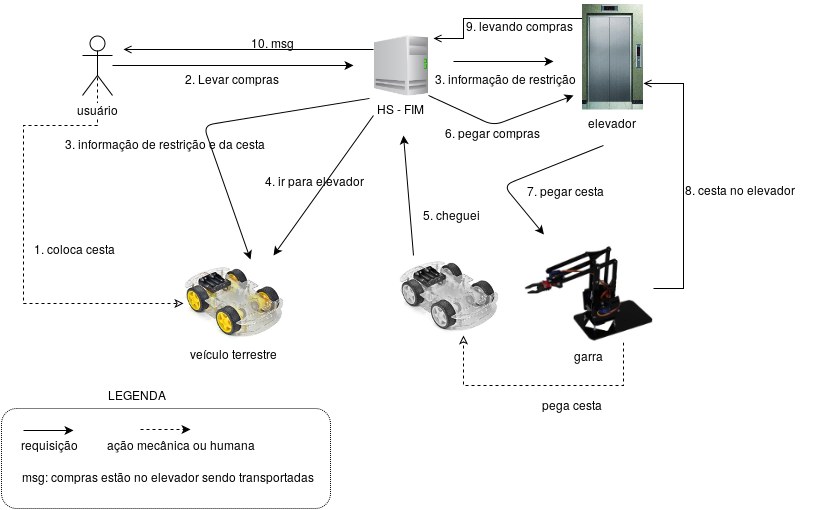
\includegraphics[width=1.0\columnwidth]{cenario_requests} 
  \caption{Cenário Levar compras.} 
  \label{fig:cenario}
\end{figure}

No cenário da Figura \ref{fig:cenario} o elevador não contém motores nem algum outro tipo de sistema elétrico ou mecânico, este é representado por uma caixa de papelão e um sensor de obstáculo acoplado. O veículo terrestre é representado por um programa carregado no Arduino UNO\footnotemark \footnotetext{\url{https://www.arduino.cc/en/Main/ArduinoBoardUno}}, o qual escuta através de sua porta serial mensagens provindas do PC (Figura \ref{fig:cenario}) e as processa simulando as funcionalidades ``Ir para elevador'' e ``cheguei''. Pela mesma porta serial o veículo terrestre encaminha suas mensagens ao PC. Os dispositivos veículo, elevador e garra podem ser visualizados na Figura \ref{fig:cenario_real}.

\begin{figure}[!htb] \centering 
  \centering
  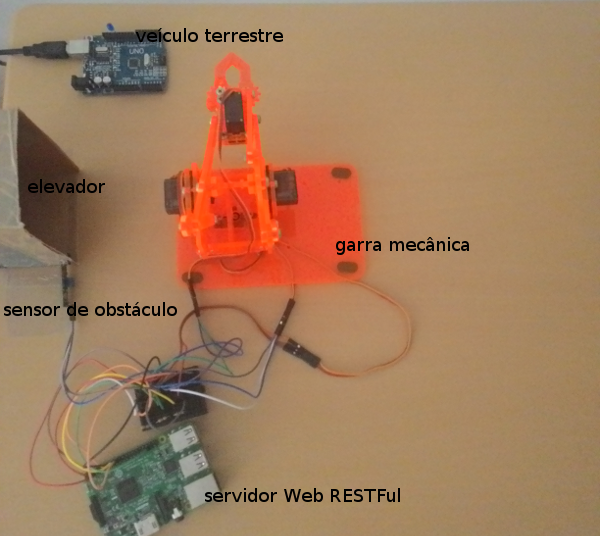
\includegraphics[width=0.8\columnwidth]{cenario_foto_real} 
  \caption{Dispositivos reais do cenário ``Levar compras''.} 
  \label{fig:cenario_real}
\end{figure}

\subsection{Execução do cenário}
De acordo com a Figura \ref{fig:cenario} o primeiro passo para inicializar a execução do cenário é colocar a cesta no veículo terrestre. Apesar do veículo ser simulado através de um software embarcado no Arduino, este necessita das informações dos objetos que se deseja transportar. Sendo assim, as informações da cesta são passadas quando o usuário executa o passo 2 (Levar compras). O usuário digita o ``id da cesta'' (no banco de dados) que se deseja transportar e clica em um botão para inicializar o serviço. Todas as cestas são compostas com miniaturas de objetos que normalmente são encontrados em supermercados, exemplos de cestas podem ser visualizados na Figura \ref{fig:exemplos_cesta}. Todos os objetos e cestas estão cadastradas no banco de dados na nuvem (amazon RDS\footnotemark \footnotetext{\url{https://aws.amazon.com/pt/rds/postgresql/}}), o qual foi apresentado na Figura \ref{fig:hnsworkmodel}. A lista de objetos que podem fazer parte de uma cesta é demonstrada na Figura \ref{fig:lista_objetos}, observe que para cada objeto é cadastrado suas características de massa, largura, comprimento, altura e diâmetro.

\begin{figure}[!htb] \centering 
  \centering
  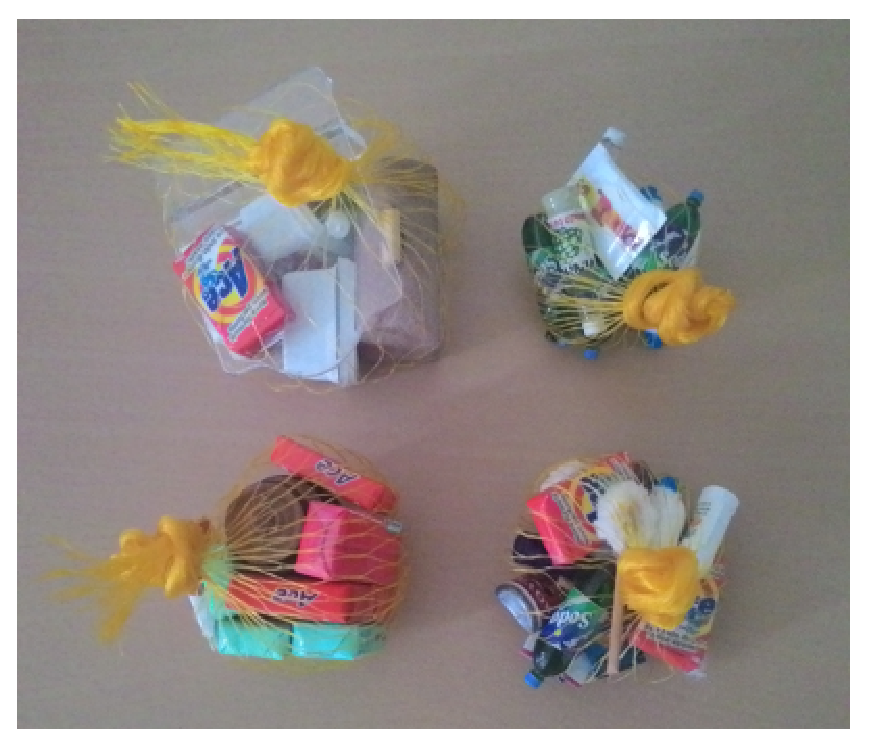
\includegraphics[width=0.8\columnwidth]{experimento/exemplos_cesta} 
  \caption{Exemplo de cestas do cenário ``Levar compras``.} 
  \label{fig:exemplos_cesta}
\end{figure}

\begin{figure}[!htb] \centering 
  \centering
  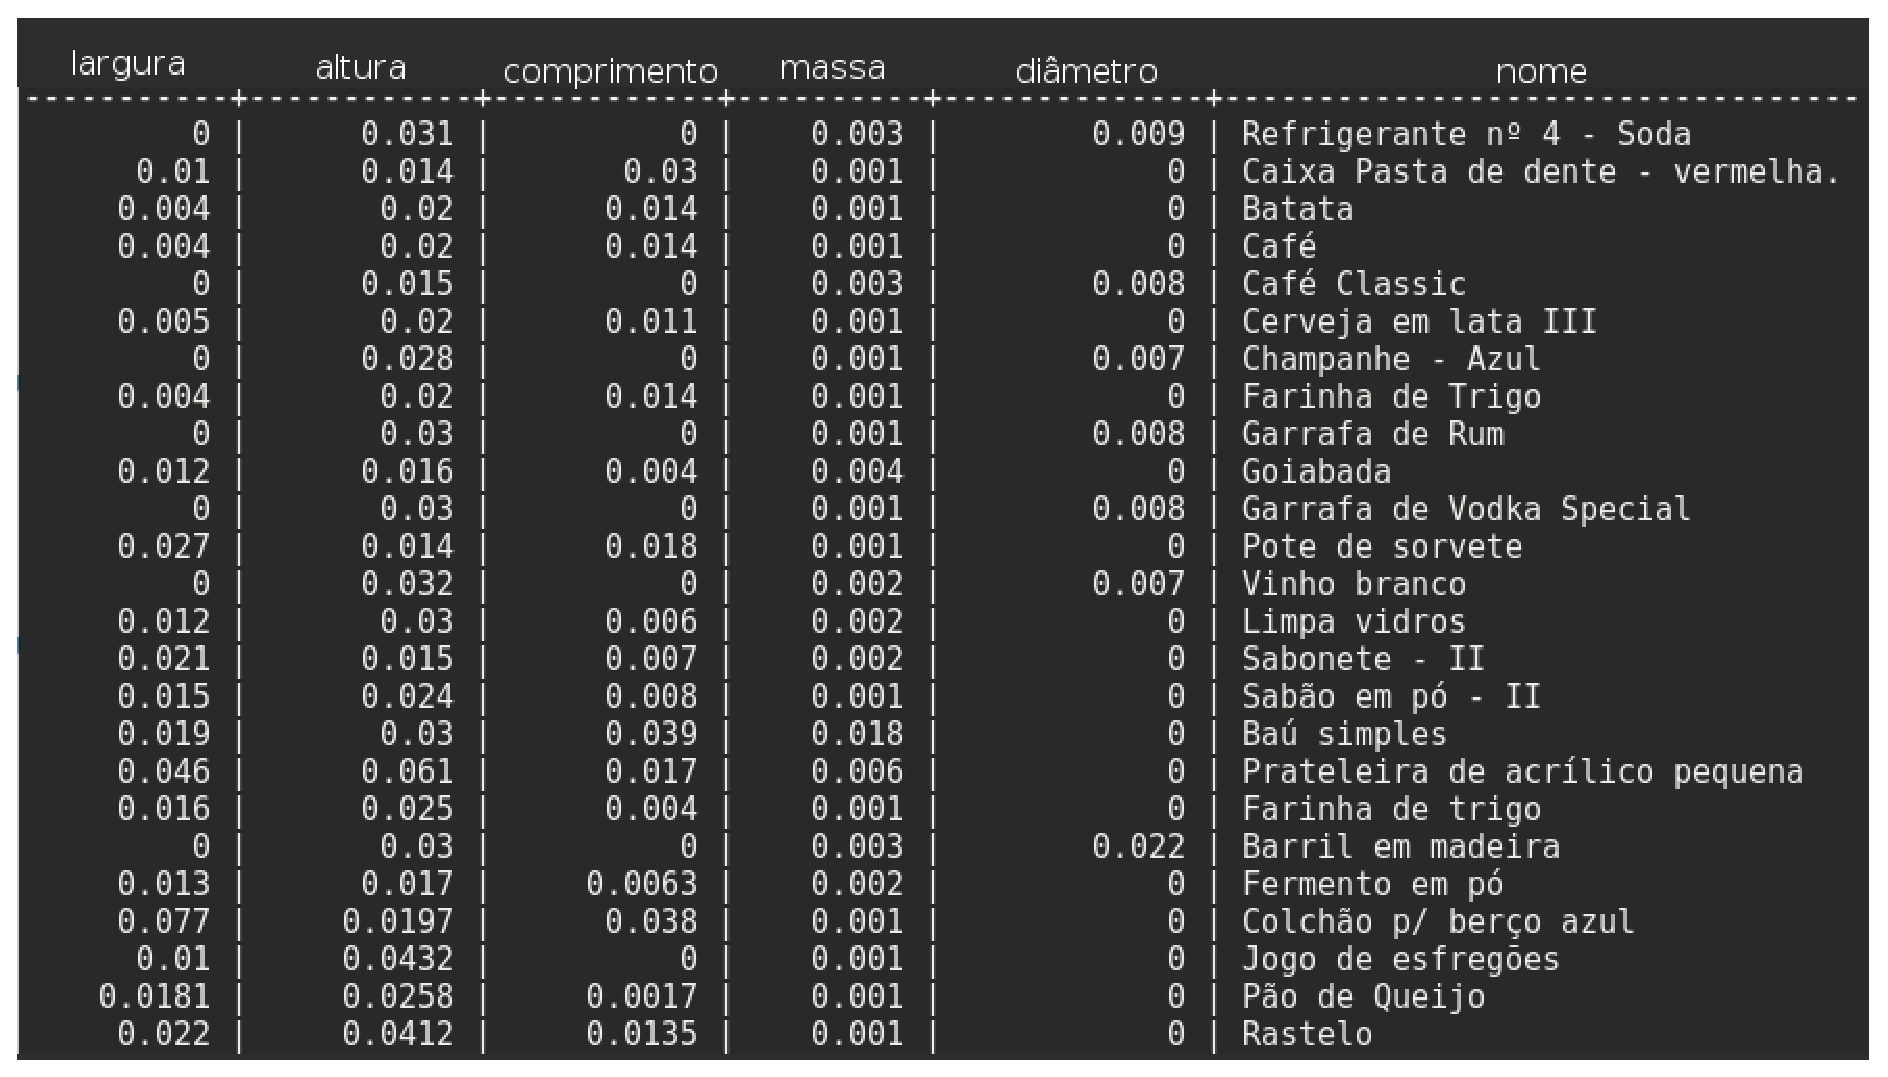
\includegraphics[width=0.8\columnwidth]{experimento/lista_items} 
  \caption{Lista dos objetos que podem ser utilizados para compor uma cesta.} 
  \label{fig:lista_objetos}
\end{figure}

Os próximos passos (3, 4, 5, e 6) do cenário podem ser executados sem mais problemas, pois já têm toda a informação necessária e não necessita de nenhuma intervenção humana. Isto já não acontece com o passo 7 (pegar cesta), pois este necessita de intervenção humana para a garra poder pegar a cesta e continuar a realizar o seu serviço, é preciso posicionar a cesta no lugar correto para a garra prender a cesta, como pode ser visto na Figura \ref{fig:garra_pegando_objeto}. Então, após a garra executar seu serviço esta manda uma mensagem para o elevador e, caso não tenha nada obstruindo a porta do elevador este inicia o transporte da cesta até o local desejado e manda uma mensagem para o fim. Daí em diante a execução do cenário continua da mesma forma com já explanado.

\begin{figure}[!htb] \centering 
  \centering
  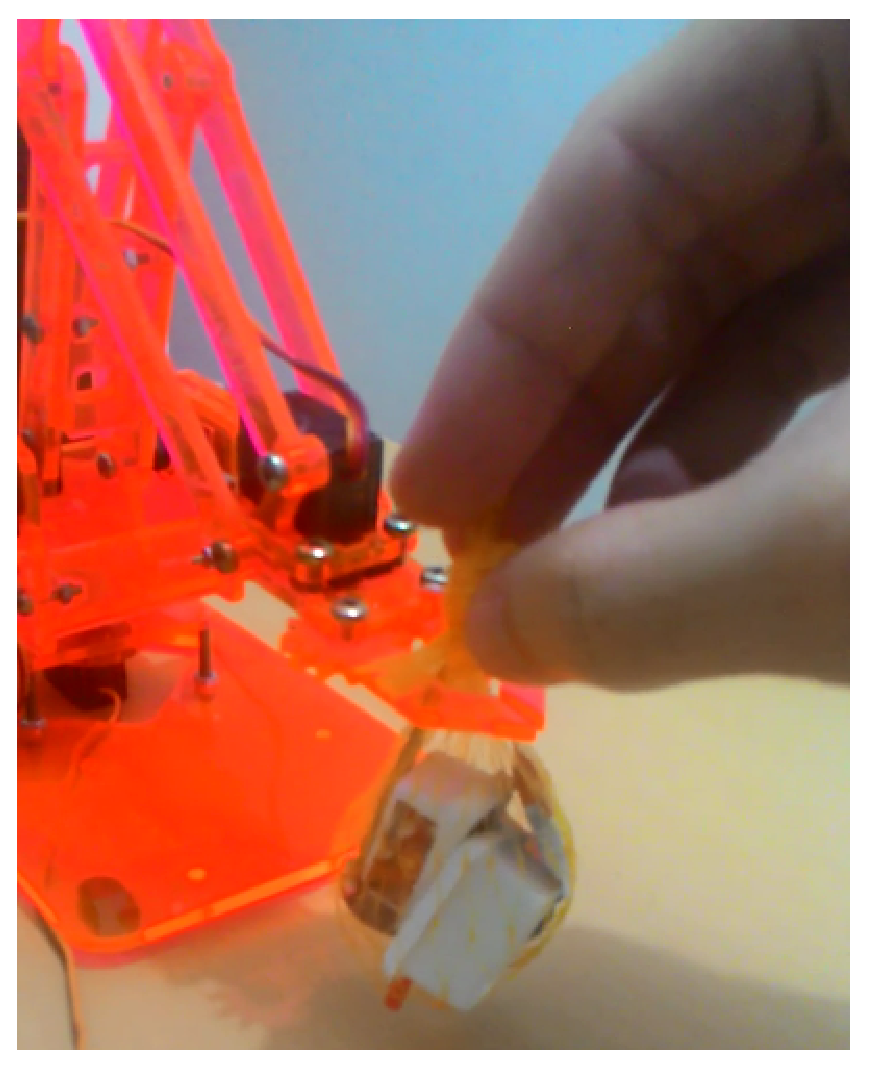
\includegraphics[width=0.8\columnwidth]{experimento/garra_pegando_objeto} 
  \caption{Cesta posicionada no local adequado por um humano, para que a garra possa prender a cesta adequadamente.} 
  \label{fig:garra_pegando_objeto}
\end{figure}

\subsection{Discussão da execução do cenário}
Para o cenário ``Levar compras`` foram confeccionadas e cadastradas no banco 66 cestas distintas. Antes de registrar as cestas no banco sempre era observado se a cesta cabia dentro do elevador quando colocadas de forma manual, e se também não ultrapassava os limites da porta, o limite de detecção do sensor de obstáculos. Então a cesta só era registrada caso coubesse no elevador e não estivesse em área que pudesse obstruir a porta. 

O cenário foi executado 66 vezes, uma para cada cesta, e pode-se observar que em algumas vezes o comportamento da garra provocava um efeito colateral indesejável (seção \ref{sec:featureinteraction}) na funcionalidade ``Levar carga'', pois a garra durante a execução do seu serviço (pegar cesta, mover de uma lado a outro , largar cesta) acabava por vezes não conseguindo que a cesta ficasse disposta dentro do elevador de uma maneira em que este pudesse continuar com o serviço de ``Levar carga'', apesar que para todos esses casos se esperava sempre como resultado o elevador levar as compras sem problemas, já que se era sabido que as cestas cabiam no elevador e, nenhuma delas feria as restrições de massa do carro nem do elevador. Tanto o veículo quanto o elevador sempre funcionaram de maneira esperada nestas execuções, pois o veículo sempre levava a carga para o local destinado avisando quando chegasse, e o elevador sempre acionava o serviço da garra, levava a carga  e avisava ao FIM quando não tinha obstáculo na porta, enquanto deixava de levar quando tinha, funcionando de maneira correta quanto as especificações de sua funcionalidade de locomoção, mas indo contra o comportamento esperado da funcionalidade pai ``Levar carga''. 

Concluindo as observações feitas até agora, o comportamento da garra junto com os tipos de objetos presentes na cesta faziam com que algumas vezes ocorressem locomoção destes durante o transporte da garra, e também no momento em que os objetos eram postos no compartimento do elevador. Nesse momento, os objetos as vezes geravam outras dimensões de cesta e/ou deslocamento da mesma, devido a natureza dos objetos e da forma como os objetos eram soltos pela garra. Sendo assim, para tentar detectar esses efeitos colaterais indesejáveis através de redes neurais, utilizou-se dos valores das grandezas físicas dos objetos (altura, massa, largura, comprimento, diâmetro) para gerar características que pudessem ser interessantes para a construção de modelos de redes neurais satisfatórios (ver seção \ref{sec:construmrn}).

Como todas as cestas estavam previamente cadastradas no banco de dados, a estas foram atribuídos valores de ``é efeito colateral'' ou ``não é efeito colateral'', a medida que se observava cada execução do cenário.

\section{Conjunto de dados - seleção dos atributos}
\label{sec:construmrn}
Os dados coletados na etapa de execução do cenário ``Levar carga'', 66 cestas, ainda estão muito brutos, observe que uma cesta deve conter pelo menos um objeto, como também pode conter muitos. Supomos que a cesta tenha 10 objetos, então o total de características da cesta seria $10.5=50$, pois cada objeto possui cinco características. Utilizar as características dos objetos desta forma, além de provavelmente não predizer nada em um modelo de rede neural, terá um custo computacional muito elevado. Para diminuir a quantidade de atributos e melhor qualificá-los gerou-se características a partir de todos os atributos dos objetos da cesta: média das alturas, dos comprimentos, das larguras, dos diâmetros e das massas, assim como o total de cada uma dessas medidas, e o total de itens. De ínicio então têm-se a seleção de 11 parâmetros.

Com a seleção prévia desses atributos, constriu-se um arquivo ``arff'', que é o tipo de arquivo padrão utilizado como \textit{dataset} pelo Weka\cite{Hall:2009}. Este \textit{dataset} é composto de 46 instâncias, cada uma com 11 atributos mais um que identifica a qual classe pertence. As outras 20 instâncias serão deixadas para um possível teste no cenário proposto, já com um classificador satisfatório, caso este seja possível de se construir.

O próximo passo utilizado nesse processo de seleção de atributos foi o de visualizar estes novos parâmetros par a par, e verificar quais pares parecem melhor separar as classes ``é efeito colateral'' ou ``não é efeito colateral''. Nas Figuras \ref{fig:plotall1}, \ref{fig:plotall2}, \ref{fig:plotall3} pode-se ter uma ideia de tal visualização. Dentre essas plotagens foram selecionadas três plotagens (Figuras \ref{fig:sl_sm}, \ref{fig:sd_sl} e \ref{fig:ma_sl}), as quais parecem melhor separar as classes, são respectivamente os pares ordenados (somaLargura, somaMassa), (somaDiâmetro, somaLargura) e (médiaAltura, somaLargura). Então, desta fase inicial de seleção dos atributos, estes foram os pares selecionados, e serão utilizados na construção de três modelos. Observe que após realizado a seleção dos atributos o espaço de \textit{features} foi reduzido a duas características.

\begin{figure}[!htb] \centering 
  \centering
  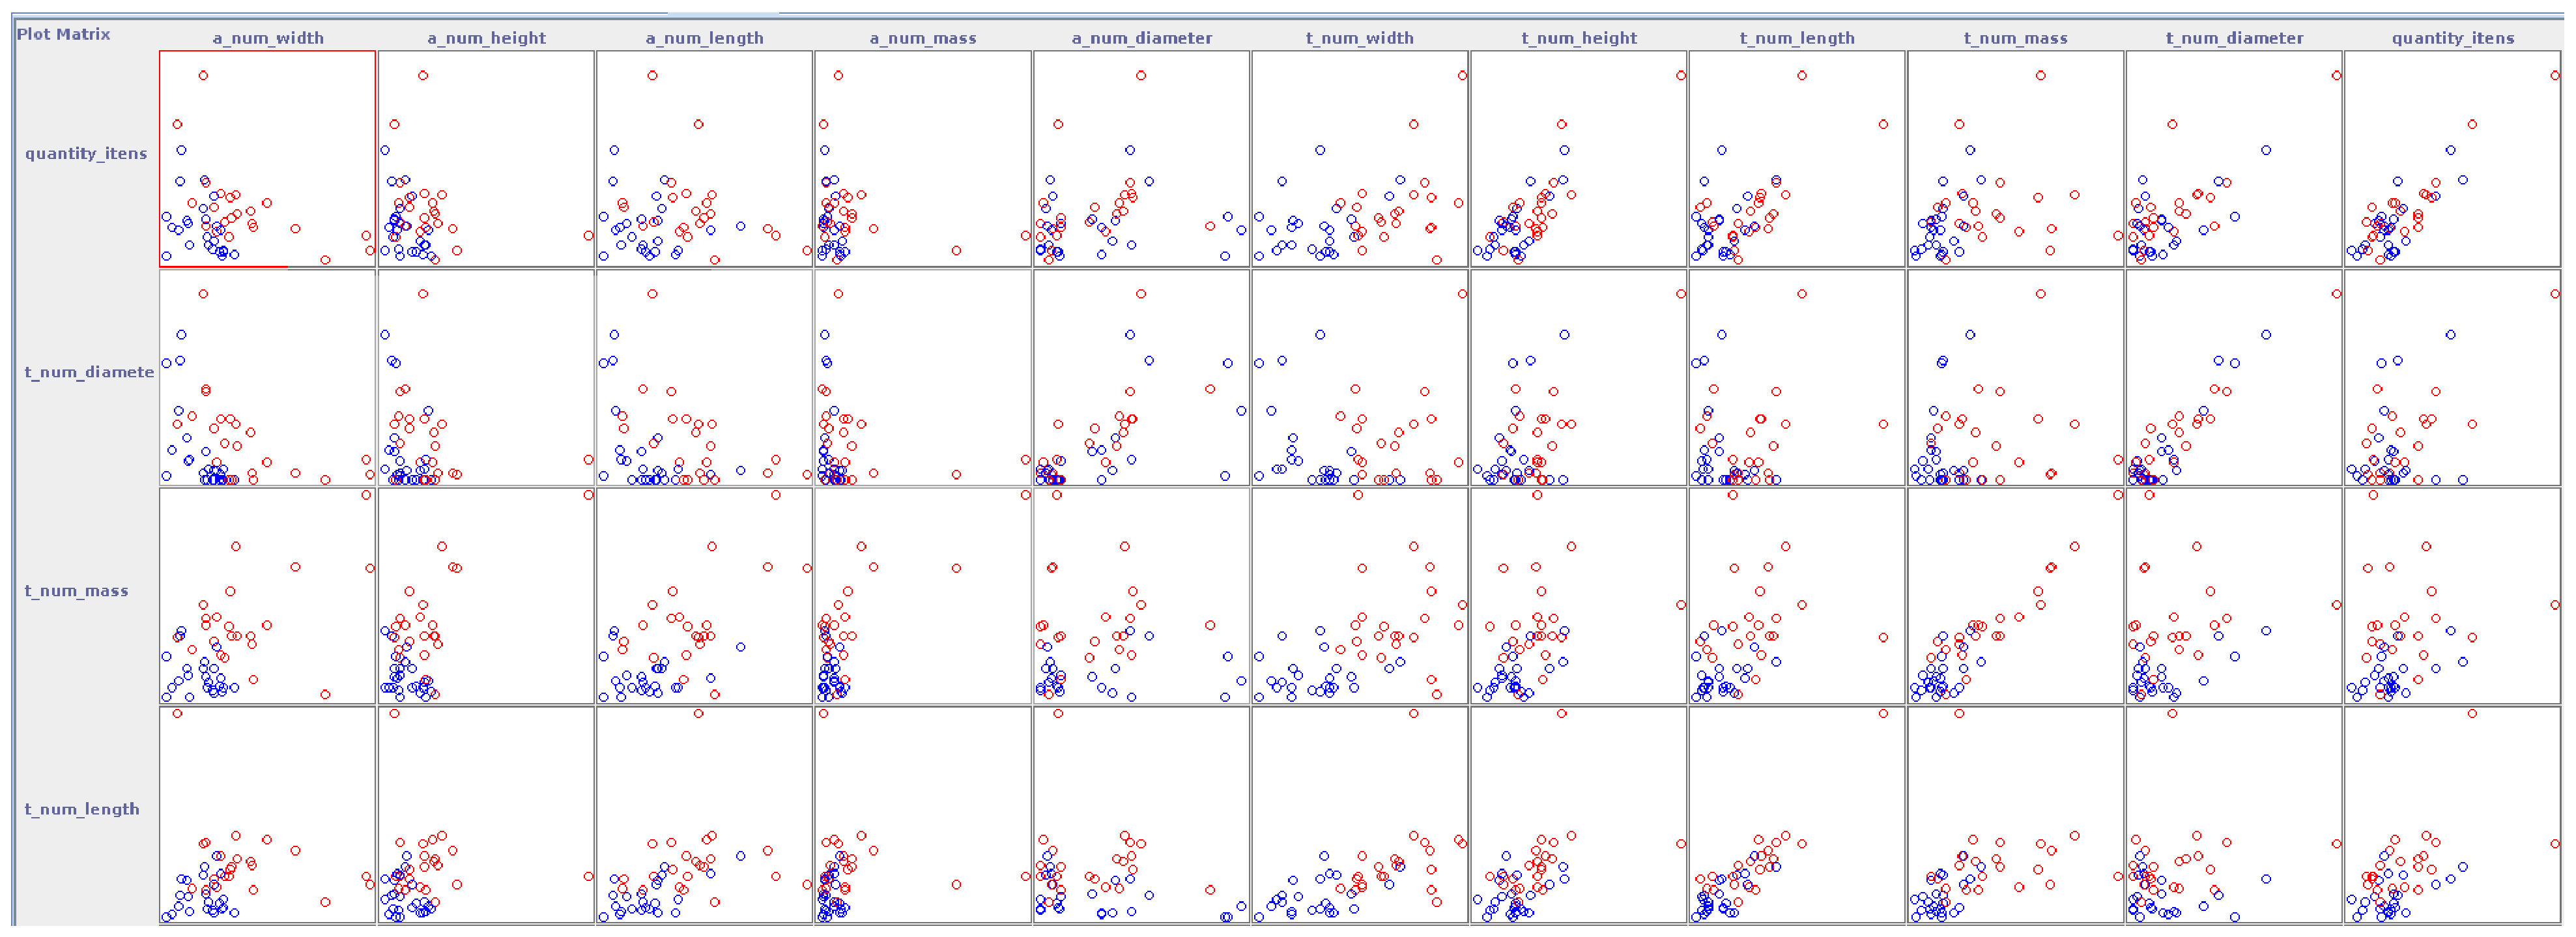
\includegraphics[width=1.0\columnwidth]{experimento/all1_plot} 
  \caption{Plotagem 1 de todas a médias e totais das características dos objetos, conjugadas par a par.} 
  \label{fig:plotall1}
\end{figure}

\begin{figure}[!htb] \centering 
  \centering
  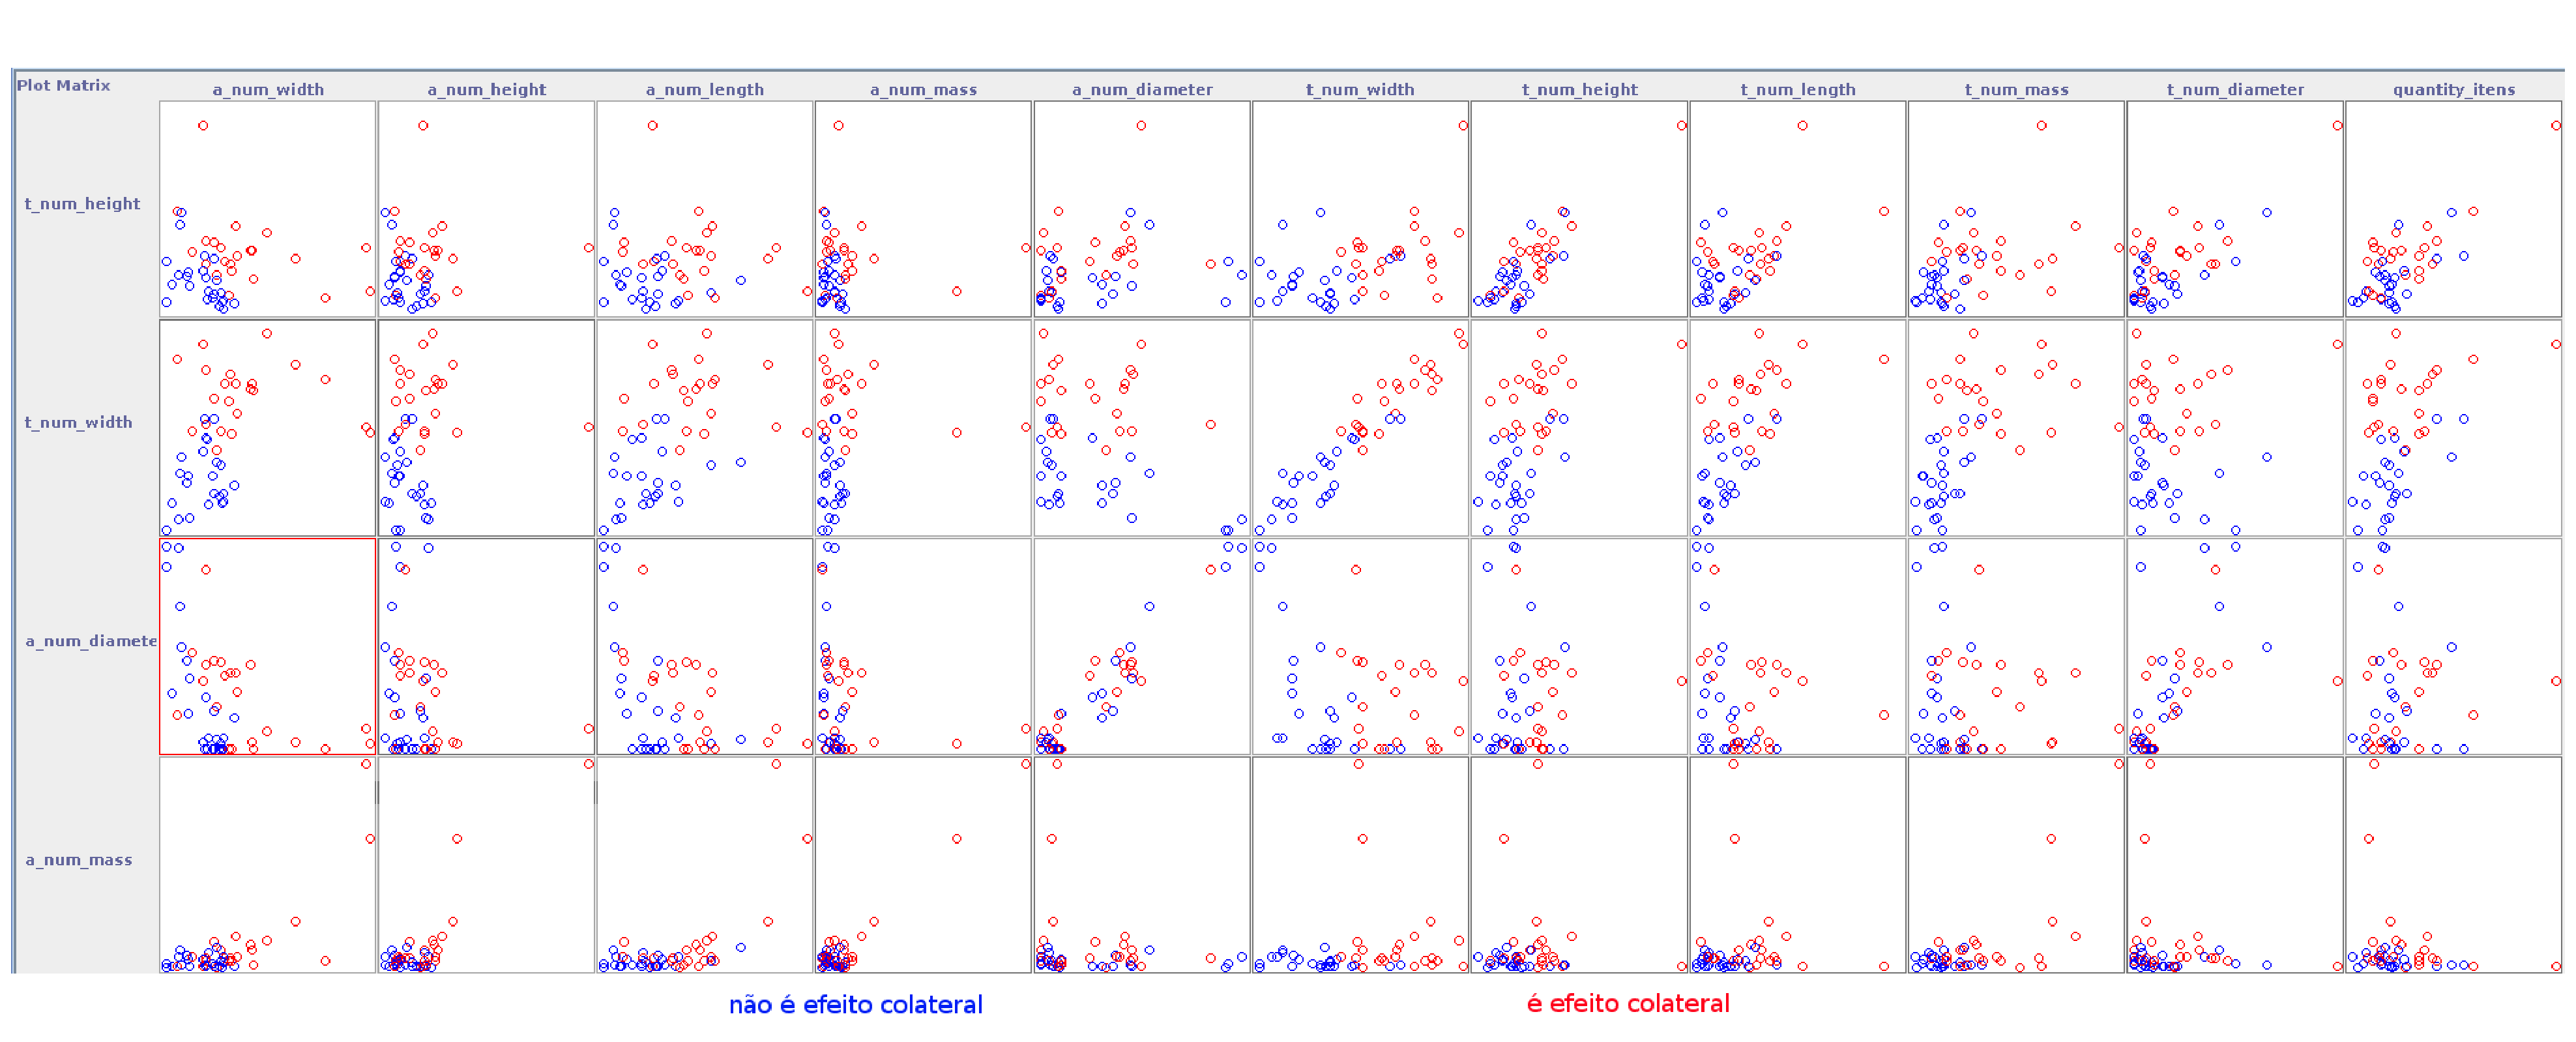
\includegraphics[width=1.0\columnwidth]{experimento/all2_plot} 
  \caption{Plotagem 2 de todas a médias e totais das características dos objetos, conjugadas par a par.} 
  \label{fig:plotall2}
\end{figure}

\begin{figure}[!htb] \centering 
  \centering
  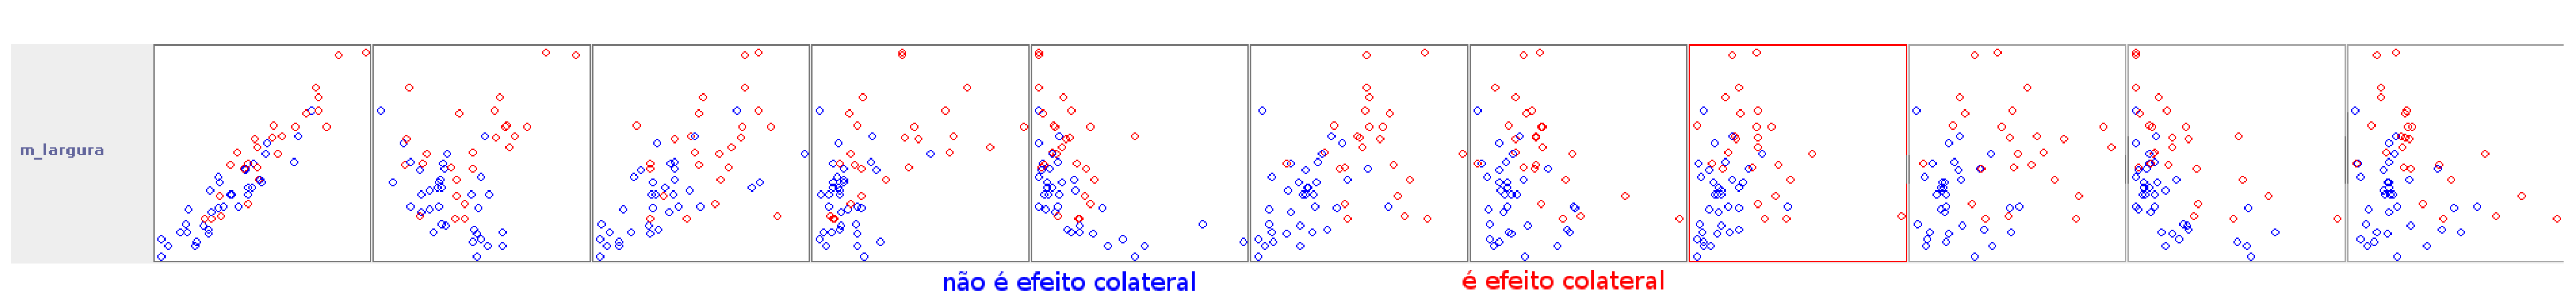
\includegraphics[width=1.0\columnwidth]{experimento/all3_plot} 
  \caption{Plotagem 3 de todas a médias e totais das características dos objetos, conjugadas par a par.} 
  \label{fig:plotall3}
\end{figure}

\begin{figure}[!htb] \centering 
  \centering
  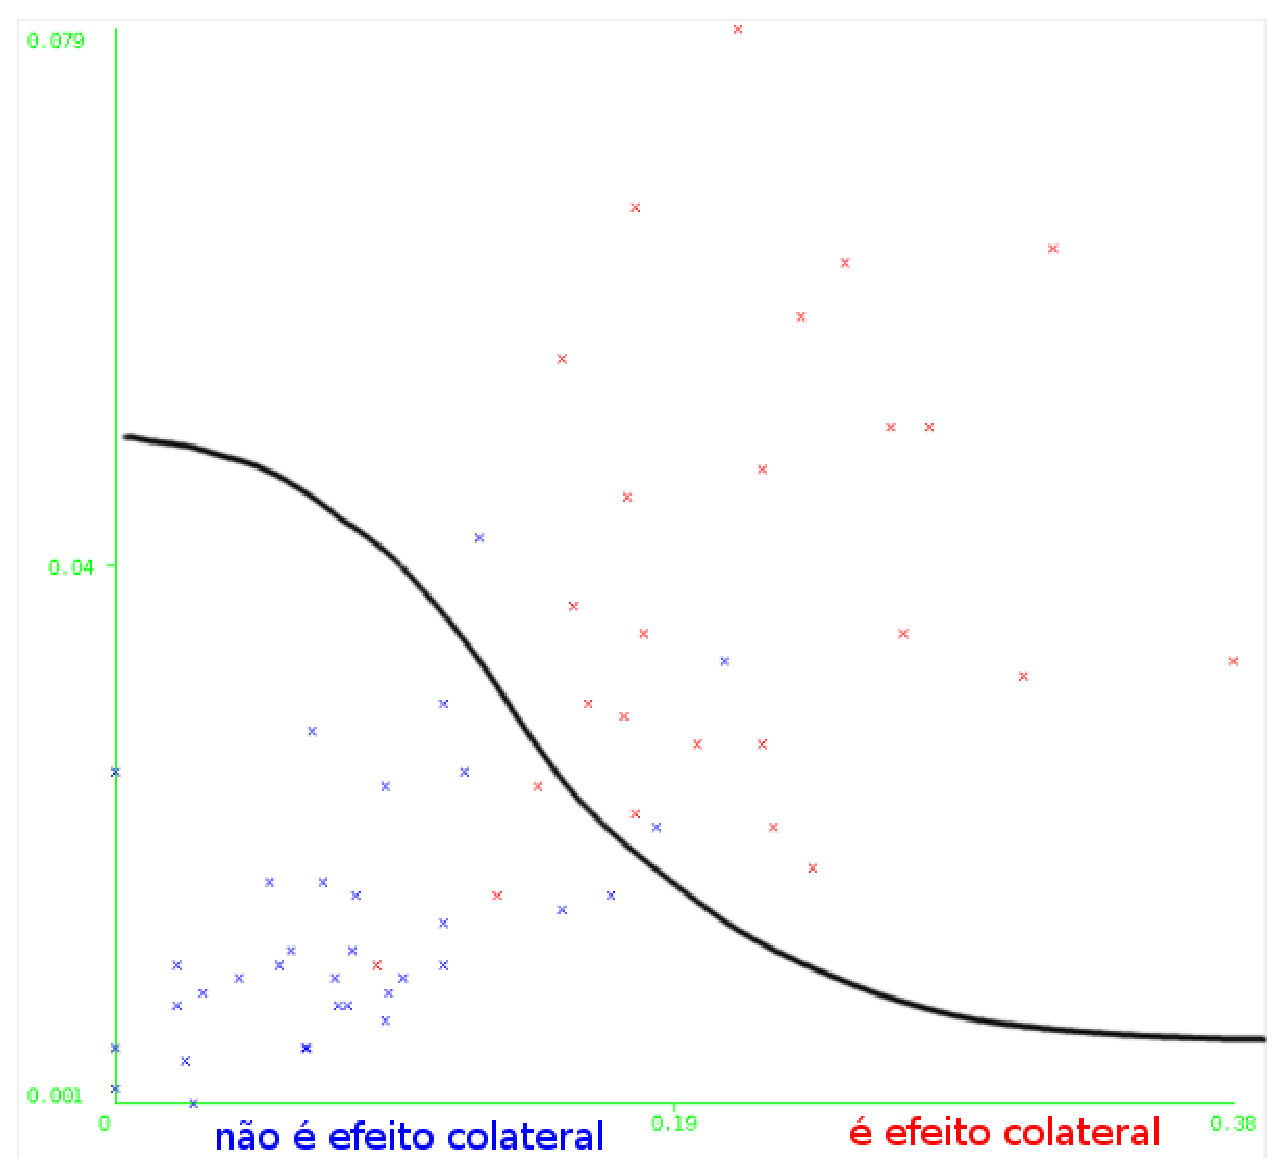
\includegraphics[width=0.8\columnwidth]{experimento/sl_sm} 
  \caption{Plotagem dos atributos (somaLargura, somaMassa). } 
  \label{fig:sl_sm}
\end{figure}

\begin{figure}[!htb] \centering 
  \centering
  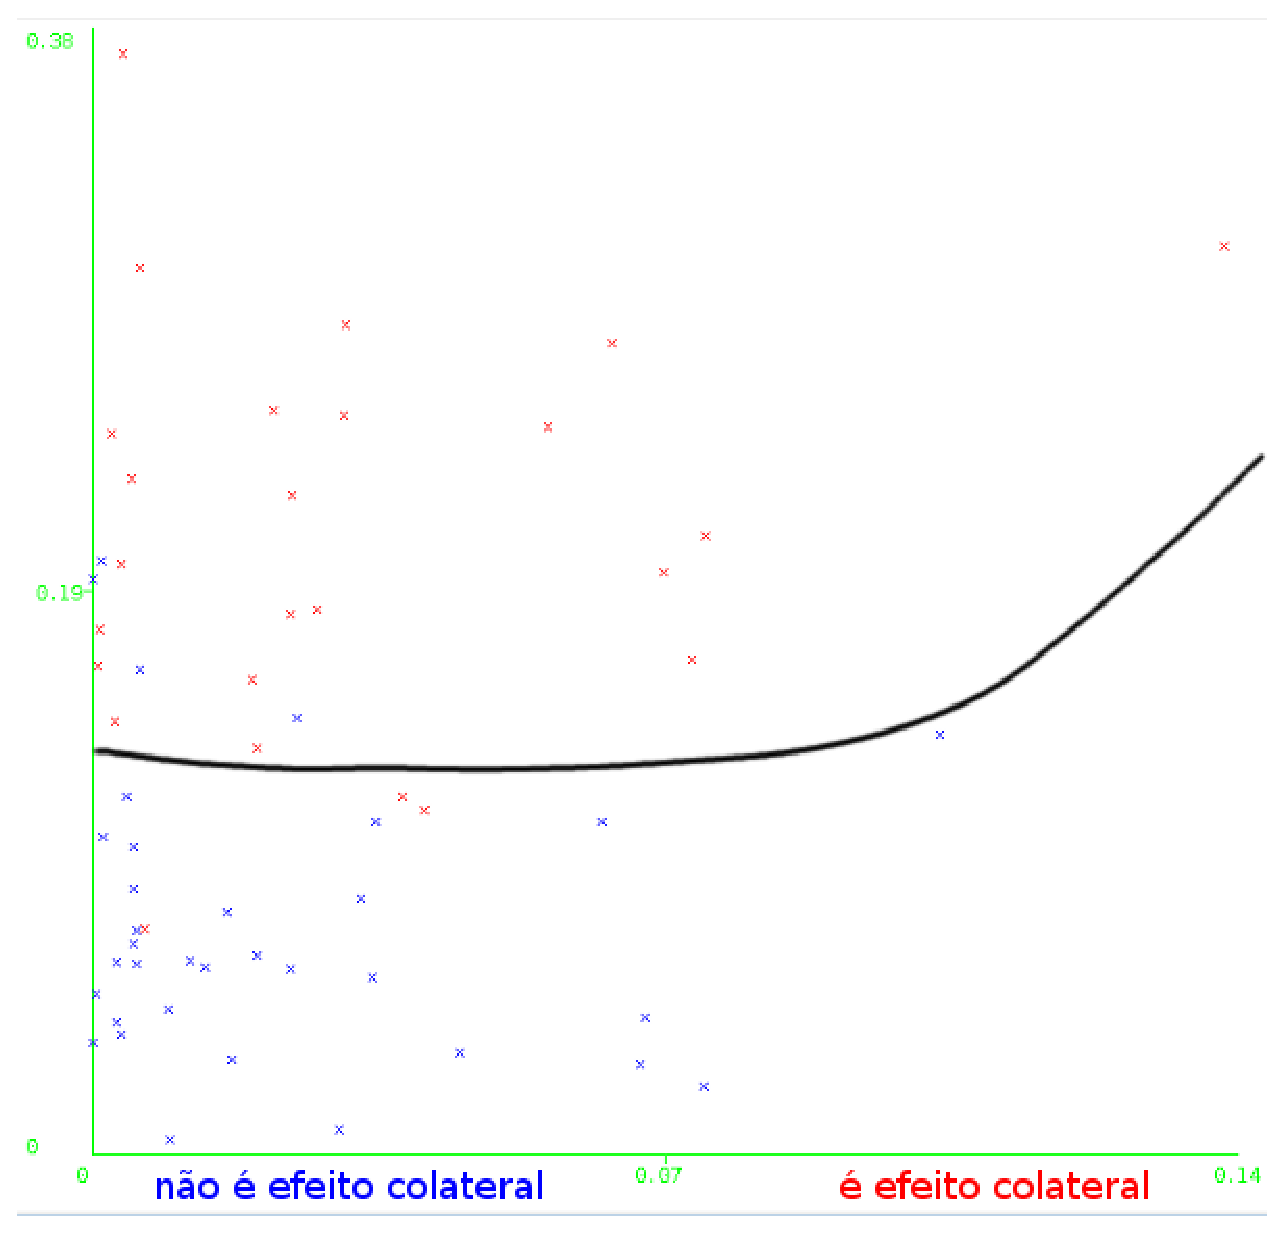
\includegraphics[width=0.8\columnwidth]{experimento/sd_sl} 
  \caption{Plotagem dos atributos (somaDiâmetro, somaLargura). } 
  \label{fig:sd_sl}
\end{figure}

\begin{figure}[!htb] \centering 
  \centering
  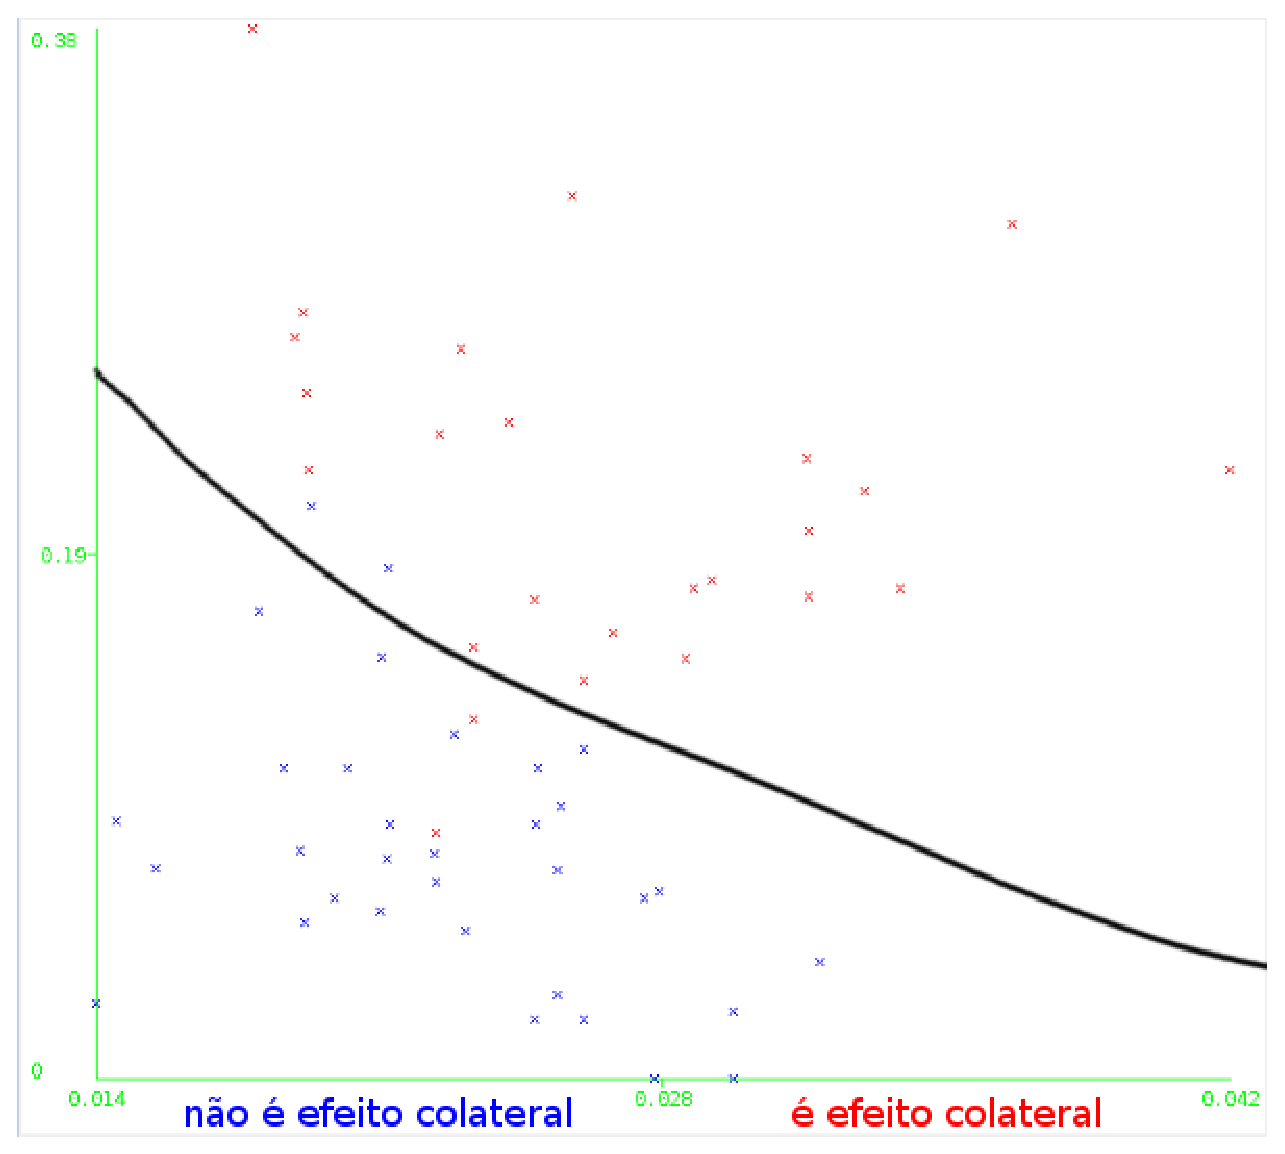
\includegraphics[width=0.8\columnwidth]{experimento/ma_sl} 
  \caption{Plotagem dos atributos (médiaAltura, somaLargura). } 
  \label{fig:ma_sl}
\end{figure}

\section{Construção e validação do modelo de redes neurais}
Para esta etapa de validação de modelo (algoritmo multilayer perceptron e \textit{dataset}) escolheu-se o método avaliativo \textit{stratified-k-fold-cross-validation}, pois este é um dos mais recomendados para bases de dados pequenas, como já discutido em \ref{subsec:evaluationMethods}. 

A justificativa de se utilizar das redes neurais como algoritmo do modelo é que além de ter resultados satisfatórios, esta se encaixa muito bem em espaço de \textit{features} não separáveis linearmente (seção \ref{sec:classificacao}), este espaço não linearmente separável pôde ser demonstrado pelas Figuras \ref{fig:plotall1}, \ref{fig:plotall2}, \ref{fig:plotall3}. A rede neural do modelo contém somente uma camada escondida (Figura \ref{fig:rede_neural_2atr}), pois é o suficiente para aproximação de qualquer função contínua\cite{Pasini:2015}, que pode ser visualizada nas figuras \ref{fig:tw_ad} e \ref{fig:tw_tm}.

\begin{figure}[!htb] \centering 
  \centering
  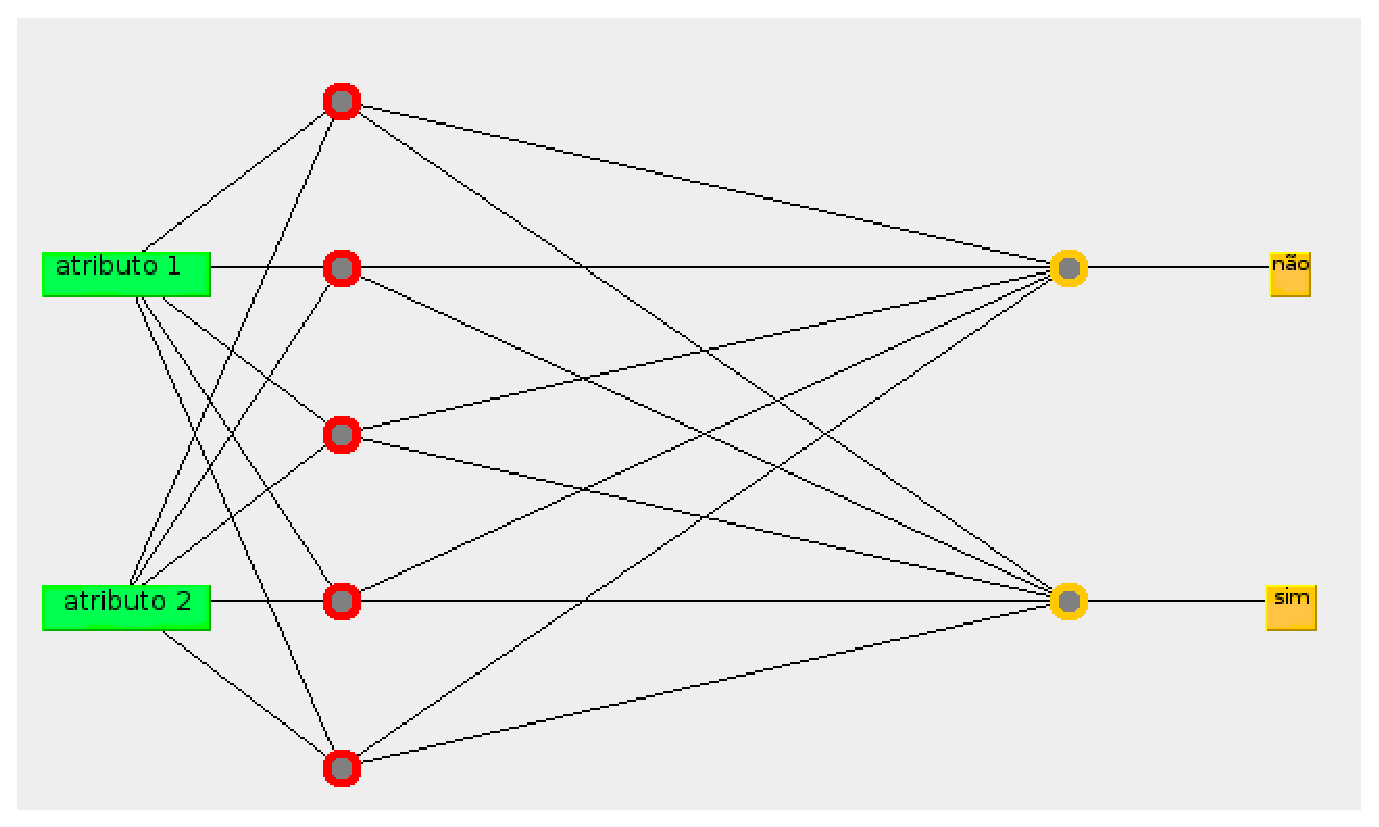
\includegraphics[width=0.8\columnwidth]{experimento/rede_neural_2atr} 
  \caption{Rede neural multilayer perceptron com uma camada escondida e dois neurônios de saída. } 
  \label{fig:rede_neural_2atr}
\end{figure}

Diante dos pares de atributos selecionados na etapa de seleção anterior (seção \ref{sec:construmrn}), utilizou-se o método \textit{stratified-k-fold-cross-validation} com a finalidade de verificar a generalização dos dois modelos e comparalá-los.

Observando um pouco mais as características dos objetos da cesta (Figura \ref{fig:lista_objetos}), percebe-se que existem objetos que não possuem nem largura nem comprimento, estes são os objetos que possuem diâmetro. Talvez somente esses pares de características não seja suficiente para se ter uma excelente generalização para cestas com características que não participaram da execução do cenário. Desta forma, após realizar os procedimentos para testar a generalização do modelo... 

\section{Resultados}

\begin{figure}[!htb] \centering 
  \centering
  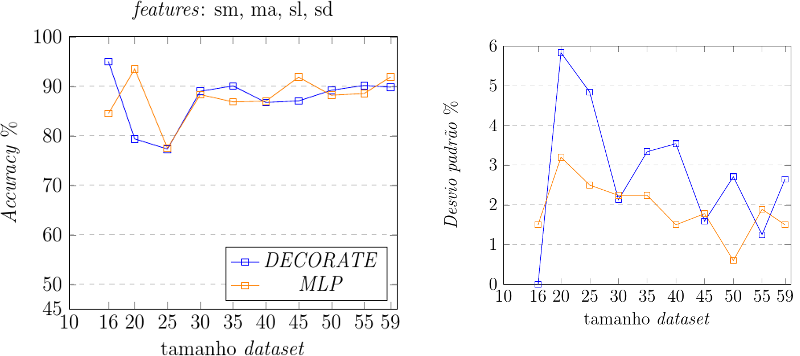
\includegraphics[width=1.0\columnwidth]{experimento/accuracy-dp_sm_ma_sl_sd} 
  \caption{Accuracy... } 
  \label{fig:accuracy_result}
\end{figure}

\begin{figure}[!htb] \centering 
  \centering
  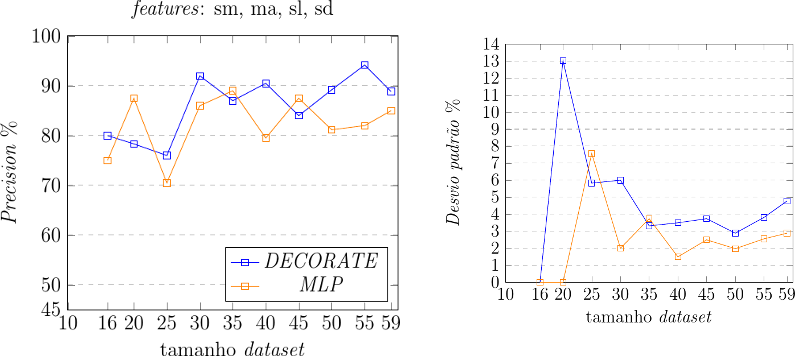
\includegraphics[width=1.0\columnwidth]{experimento/precision-dp_sm_ma_sl_sd} 
  \caption{Precision... } 
  \label{fig:precision_result}
\end{figure}

\begin{figure}[!htb] \centering 
  \centering
  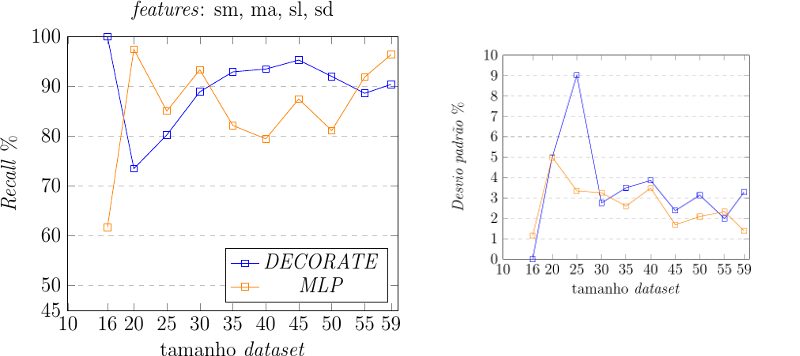
\includegraphics[width=1.0\columnwidth]{experimento/recall-dp_sm_ma_sl_sd} 
  \caption{Recall... } 
  \label{fig:recall_result}
\end{figure}

%\begin{tikzpicture}
%\begin{axis}[
 %   title={\textit{features}: sm, ma, sl, sd},
  %  xlabel={tamanho \textit{dataset}},
   % ylabel={\textit{Accuracy} \%},
    %xmin=10, xmax=60,
    %ymin=45, ymax=100,
    %xtick={10,16,20,25,30,35,40,45,50,55,59},
    %ytick={45,10,20,30,40,50,60,70,80,90,100},
    %legend pos=south east ,
    %ymajorgrids=true,
    %grid style=dashed,
%]
 
%\addplot[
 %   color=blue,
  %  mark=square,
   % ]
    %coordinates {
     % (16,95)(20,79.38)(25,77.33)(30,89)(35,90.08)(40,86.75)(45,87.05)(50,89.2)(55,90.18)(59,89.83)
    %};

%\addplot[
 %   color=orange,
  %  mark=square,
   % ]
    %coordinates {
     % (16,84.5)(20,93.5)(25,77.5)(30,88.33)(35,86.86)(40,87)(45,91.85)(50,88.2)(55,88.55)    (59,91.86)
    %};

%\legend{\textit{DECORATE},\textit{MLP}}
 
%\end{axis}
%\end{tikzpicture}

%\begin{tikzpicture}
%\begin{axis}[
 %   title={\textit{features}: sm, ma, sl, sd},
  %  xlabel={tamanho \textit{dataset}},
   % ylabel={\textit{Precision} \%},
    %xmin=10, xmax=60,
    %ymin=45, ymax=100,
    %xtick={10,16,20,25,30,35,40,45,50,55,59},
    %ytick={45,10,20,30,40,50,60,70,80,90,100},
    %legend pos=south east ,
    %ymajorgrids=true,
    %grid style=dashed,
%]
 
%\addplot[
 %   color=blue,
  %  mark=square,
   % ]
    %coordinates {
     % (16,80)(20,78.33)(25,76)(30,92)(35,87)(40,90.5)(45,84)(50,89.2)(55,94.17)(59,88.83)
    %};

%\addplot[
 %   color=orange,
  %  mark=square,
   % ]
    %coordinates {
     % (16,75)(20,87.5)(25,70.5)(30,86)(35,89)(40,79.5)(45,87.5)(50,81.17)(55,82)(59,85)
    %};

%\legend{\textit{DECORATE},\textit{MLP}}
 
%\end{axis}
%\end{tikzpicture}

%\begin{tikzpicture}
%\begin{axis}[
 %   title={\textit{features}: sm, ma, sl, sd},
  %  xlabel={tamanho \textit{dataset}},
   % ylabel={\textit{Recall} \%},
    %xmin=10, xmax=60,
    %ymin=45, ymax=100,
    %xtick={10,16,20,25,30,35,40,45,50,55,59},
    %ytick={45,10,20,30,40,50,60,70,80,90,100},
    %legend pos=south east ,
    %ymajorgrids=true,
    %grid style=dashed,
%]
 
%\addplot[
 %   color=blue,
  %  mark=square,
   % ]
    %coordinates {
     % (16,100)(20,73.52)(25,80.29)(30,88.96)(35,92.96)(40,93.52)(45,95.33)(50,92.05)(55,88.65)(59,90.44)
    %};

%\addplot[
 %   color=orange,
  %  mark=square,
   % ]
    %coordinates {
     % (16,61.75)(20,97.5)(25,85.08)(30,93.39)(35,82.19)(40,79.5)(45,87.5)(50,81.17)(55,91.93)(59,96.43)
    %};

%\legend{\textit{DECORATE},\textit{MLP}}
 
%\end{axis}
%\end{tikzpicture}

%\begin{tikzpicture}%desvio padrão accuracy
%\begin{axis}[
    %title={\textit{features}: sm, ma, sl, sd},
 %   xlabel={tamanho \textit{dataset}},
  %  ylabel={\textit{Desvio padrão} \%},
   % xmin=10, xmax=60,
    %ymin=0, ymax=6,
    %xtick={10,16,20,25,30,35,40,45,50,55,59},
    %ytick={0,1,2,3,4,5,6},
    %legend pos=north east ,
    %ymajorgrids=true,
    %grid style=dashed,
%]
 
%\addplot[
 %   color=blue,
  %  mark=square,
   % ]
    %coordinates {
     % (16,0)(20,5.83)(25,4.84)(30,2.13)(35,3.34)(40,3.54)(45,1.59)(50,2.71)(55,1.25)(59,2.65)
    %};

%\addplot[
 %   color=orange,
  %  mark=square,
   % ]
    %coordinates {
     % (16,1.5)(20,3.2)(25,2.5)(30,2.24)(35,2.24)(40,1.5)(45,1.78)(50,0.6)(55,1.89)(59,1.5)
    %};
 
%\end{axis}
%\end{tikzpicture}

%\begin{tikzpicture}%desvio padrão precision
%\begin{axis}[
    %title={\textit{features}: sm, ma, sl, sd},
 %   xlabel={tamanho \textit{dataset}},
  %  ylabel={\textit{Desvio padrão} \%},
   % xmin=10, xmax=60,
    %ymin=0, ymax=14,
    %xtick={10,16,20,25,30,35,40,45,50,55,59},
    %ytick={0,1,2,3,4,5,6,7,8,9,10,11,12,13,14},
    %legend pos=north east ,
    %ymajorgrids=true,
    %grid style=dashed,
%]
 
%\addplot[
 %   color=blue,
  %  mark=square,
   % ]
    %coordinates {
     % (16,0)(20,13.02)(25,5.83)(30,6)(35,3.32)(40,3.5)(45,3.74)(50,2.89)(55,3.82)(59,4.78)
    %};

%\addplot[
 %   color=orange,
  %  mark=square,
   % ]
    %coordinates {
     % (16,0)(20,0)(25,7.57)(30,2)(35,3.74)(40,1.5)(45,2.5)(50,1.98)(55,2.56)(59,2.89)
    %};
 
%\end{axis}
%\end{tikzpicture}

%\begin{tikzpicture}%desvio padrão recall
%\begin{axis}[
    %title={\textit{features}: sm, ma, sl, sd},
 %   xlabel={tamanho \textit{dataset}},
  %  ylabel={\textit{Desvio padrão} \%},
   % xmin=10, xmax=60,
    %ymin=0, ymax=10,
    %xtick={10,16,20,25,30,35,40,45,50,55,59},
    %ytick={0,1,2,3,4,5,6,7,8,9,10},
    %legend pos=north east ,
    %ymajorgrids=true,
    %grid style=dashed,
%]
 
%\addplot[
 %   color=blue,
  %  mark=square,
   % ]
    %coordinates {
     % (16,0)(20,4.99)(25,9.02)(30,2.76)(35,3.5)(40,3.86)(45,2.38)(50,3.14)(55,1.99)(59,3.29)
    %};

%\addplot[
 %   color=orange,
  %  mark=square,
   % ]
    %coordinates {
     % (16,1.15)(20,5)(25,3.35)(30,3.26)(35,2.6)(40,3.49)(45,1.69)(50,2.09)(55,2.33)(59,1.39)
    %};
 
%\end{axis}
%\end{tikzpicture}
